\documentclass[MoviesApp.tex]{subfiles}


\begin{document}

\section{Movie Application}

For this part of the project we were asked to implement a simple movie application lookup from an existing movie XML database. Figure \ref{fig:movieapp} below shows a screenshot of the movie application running on the eXist environment. The application was written in the eXist IDE environment and all the code for this application can be found on GitHub link.

\begin{figure} [H]
	\centering
	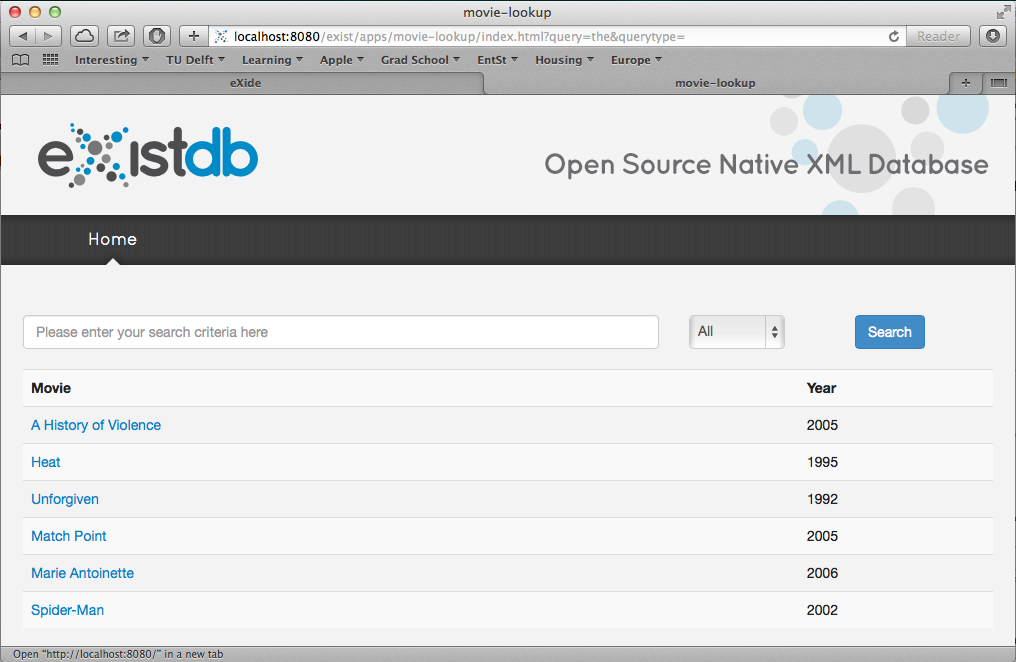
\includegraphics[width=1\textwidth]{./Figures/MovieApp.png}
	\caption{Screenshot of Movie Application}
	\label{fig:movieapp}
\end{figure}

\subsection{Search Criteria}
The search bar for the sample application allows users to search movies with the following criteria:

\begin{itemize}
\item All
\item Title
\item Keywords
\item Year
\item Director
\item Actor
\item Genre
\end{itemize}

\subsection{Selecting Movie From Returned Results}
If a matching movie(s) is found, a list is returned. More details about the movie can be found if the user clicks on the movie as shown in Figure \ref{fig:movieappselected}.

\begin{figure} [H]
	\centering
	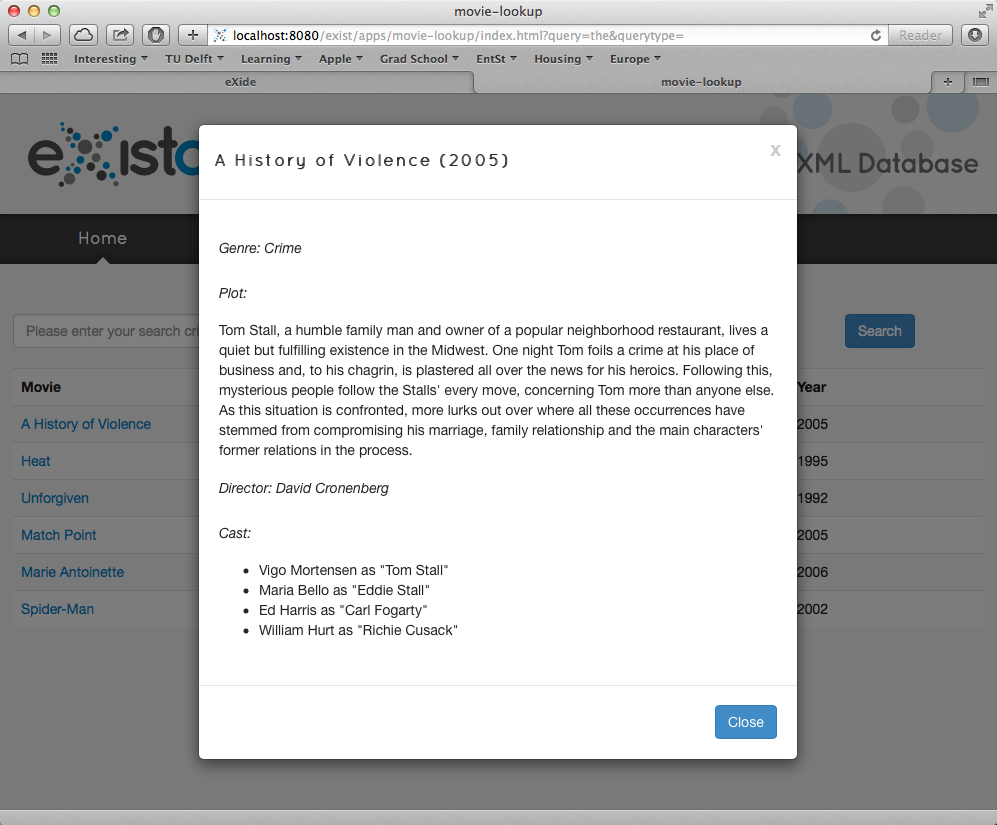
\includegraphics[width=1\textwidth]{./Figures/MovieAppSelected.png}
	\caption{Additional Movie Information}
	\label{fig:movieappselected}
\end{figure}

\end{document}